\chapter{Introducción específica} % Main chapter title

\label{Chapter2}

%----------------------------------------------------------------------------------------
%	Chapter 2
%----------------------------------------------------------------------------------------

Este capítulo lista los requerimientos y en base a ellos presenta y describe los componentes internos del sistema desarrollado, junto con las tecnologías y recursos de software utilizados para su implementación. Asimismo, se realiza una descripción simplificada del funcionamiento de un EDFA.

\section{Requerimientos}
\label{sec:reqs}

Los requerimientos fueron determinados en conjunto con la empresa en base a las funcionalidades y prestaciones con las que debe contar el sistema. Como la lista es muy extensa, se listan a continuación solamente algunos de los principales:

\renewcommand{\labelenumii}{\arabic{enumi}.\arabic{enumii}}

\begin{enumerate}

\item Encendido y apagado del EDFA
	\begin{enumerate}
	\item El software debe apagar la salida óptica del dispositivo 			EDFA bajo prueba cuando se detecte la activación de alguna de las 		alarmas.
	\item Mediante la función táctil de la pantalla LCD el usuario 			debe poder prender y apagar la alimentación del dispositivo EDFA 		bajo prueba y su salida óptica.
	\item El software debe cortar la alimentación del dispositivo EDFA 	bajo prueba cuando se detecte que la corriente supera el valor 			previamente definido.
	\item El software debe medir y mostrar en pantalla los valores de 		tensión de alimentación y consumo de corriente del dispositivo 			EDFA bajo prueba mediante las señales analógicas de entrada 			provenientes de los respectivos monitores, con una precisión no 		menor al 10\% (máximo desvío con respecto al valor real). Este 			valor debe ser de una cifra significativa para la parte entera y 		dos para la decimal.
	\end{enumerate}

\item Pantalla LCD
	\begin{enumerate}
	\item El software debe actualizar la imagen de la pantalla cada 		medio segundo (2 cuadros por segundo).
	\item La pantalla deberá indicar el estado de la salida óptica del 	dispositivo EDFA bajo prueba y el del relé de alimentación.
	\item Mediante la función táctil de la pantalla LCD el usuario 			debe poder cambiar el valor para el cual se detecta una 				sobrecorriente. El rango válido para este valor debe ser de 0 A a 		3 A, siendo la parte decimal de dos cifras significativas.
	\end{enumerate}
	
\item Entradas y salidas del EDFA
	\begin{enumerate}
	\item El software deberá mostrar en la pantalla los estados de todas las señales digitales de entrada y salida del dispositivo EDFA bajo prueba.
	\end{enumerate}

\item Requisitos de rendimiento
	\begin{enumerate}
	\item \label{item:req1} La apertura del relé de alimentación del dispositivo EDFA 		bajo prueba deberá efectuarse en un tiempo menor a 50 ms luego de 		detectarse una sobrecorriente o una caída de la tensión de 				alimentación.
	\item \label{item:req2} El apagado de la salida óptica del dispositivo EDFA bajo 			prueba deberá efectuarse en un tiempo menor a 100 ms luego de 			detectarse la activación de una alarma.
	\end{enumerate}
	
\end{enumerate}

La lista completa de requerimientos se puede ver en \citep{DOC_REQ}.

\section{Funcionamiento de un amplificador óptico}
\label{sec:funcAmp}

Los amplificadores de fibra dopados con erbio son los amplificadores ópticos más importantes en el contexto de comunicaciones ópticas de larga distancia. Son utilizados en la banda L y C del espectro (aproximadamente entre 1530 nm y 1625 nm \citep{WEBSITE:BANDAS}), región en la que las pérdidas en la fibra óptica son menores. Esto se puede ver en la figura \ref{fig:espectro}, que muestra las pérdidas en función de la longitud de onda de la luz utilizada.

\begin{figure}[H]
\centering
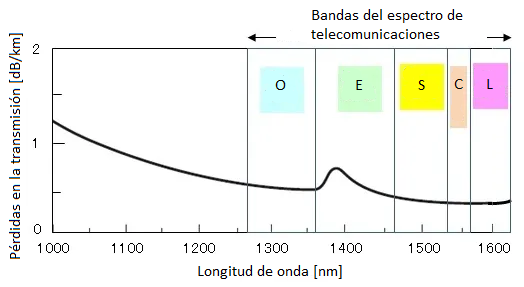
\includegraphics[width=0.85\textwidth]{./Figures/espectro.png}
\caption{Pérdidas en la fibra\protect\footnotemark.}
\label{fig:espectro}
\end{figure}

\footnotetext{Imagen tomada de \citep{WEBSITE:BANDAS}}

Inventado en 1987 \citep{WEBSITE:EDFA1}, el EDFA es generalmente usado para compensar las pérdidas mencionadas en una línea de transmisión óptica. Este puede ser colocado en tres partes: 

\begin{itemize}
\item Inmediatamente después del transmisor, para aumentar la potencia inyectada en la línea.
\item En el medio del camino óptico, para compensar las pérdidas por la distancia recorrida.
\item Antes del receptor, para favorecer la detección de la señal.
\end{itemize}

La figura \ref{fig:EDFAinterno} muestra la configuración interna más común de un EDFA. Su componente principal es la fibra dopada con erbio (EDF por sus siglas en inglés), que generalmente es monomodo \citep{WEBSITE:FIBRA}. 

La luz ingresa al amplificador mediante el puerto de entrada y luego mediante un divisor se redirige un porcentaje de la señal (generalmente entre un 1\% y 2\% \citep{WEBSITE:EDFA2}) a un detector para realizar una medición de la potencia óptica. Luego, pasa por un aislador óptico que permite la transmisión de luz en un solo sentido y así evita una realimentación debida a reflexiones en etapas posteriores.

La bomba de 980 nm es un diodo láser que genera una señal lumínica en esa longitud de onda. Esta luego se mezcla con la señal de luz entrante (a la salida del aislador) y atraviesan la fibra dopada con erbio. En esta instancia es donde se genera la amplificación de la señal propiamente dicha, mediante un efecto denominado emisión estimulada \citep{WEBSITE:EDFA2}\citep{WEBSITE:EMISSION}.

\begin{figure}[H]
\centering
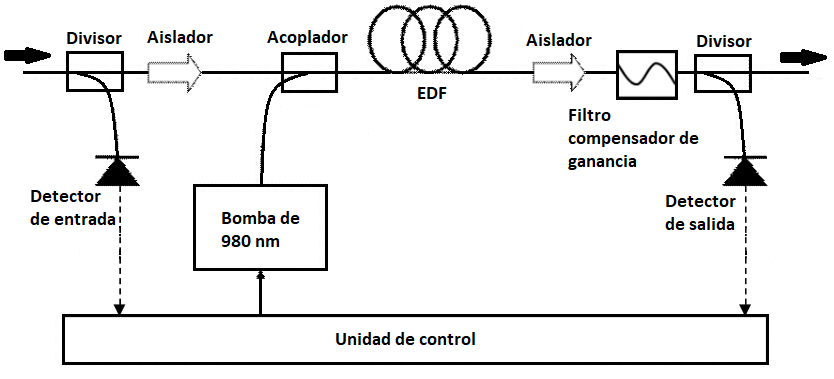
\includegraphics[width=0.85\textwidth]{./Figures/EDFAinterno.png}
\caption{Configuración interna de un EDFA\protect\footnotemark.}
\label{fig:EDFAinterno}
\end{figure}

\footnotetext{Imagen tomada de \citep{WEBSITE:EDFA2}}

Una vez amplificada, la señal pasa nuevamente por otro aislador que se encarga principalmente de filtrar la luz de 980 nm, evitando que se introduzca en el camino óptico. Luego, la señal pasa por un filtro aplanador de ganancia (GFF por sus siglas en inglés) cuyo objetivo es hacer constante la ganancia del amplificador en todo el ancho de banda de trabajo \citep{WEBSITE:EDFA3} (bandas C y L del espectro). Finalmente, antes de que la luz salga del amplificador, se realiza nuevamente una medición de la potencia óptica al igual que en la entrada.

Tanto la bomba de 980 nm como ambos detectores de potencia se encuentran conectados a una unidad de control. Esta generalmente cuenta con un microcontrolador o chip dedicado que se encarga de regular la potencia que entrega la bomba en base a los valores medidos por los detectores, creando un lazo de control automático de ganancia \citep{WEBSITE:EDFA2}\citep{WEBSITE:EDFA1}.

\section{Interfaz del amplificador óptico}
\label{sec:intAmp}

Como se mencionó en la sección \ref{sec:contexto}, para poder controlarlo, el EDFA cuenta con un conector de 25 pines tipo Micro-D \citep{WEBSITE:MICROD_DS}. Este conector contiene varios grupos de señales con distintas funciones. La tabla \ref{tab:señalesConector} lista cada una de las señales de la interfaz, junto con los detalles de su dirección, tipo y función.

\begin{table}[H]
	\centering
	\caption{Señales de la interfaz del EDFA.}
	\begin{tabular}{l c p{1.5cm} p{5cm}}
		\toprule
		\textbf{Nombre de la señal}	& \textbf{Dirección}	& \textbf{Tipo} & \textbf{Función} \\
		\midrule
		5 V 					& Entrada	& Potencia			& Entrada de alimentación del EDFA. \\		
		PGND				& Salida	& Potencia  		& Retorno de alimentación (potencia). \\
		GND					& Salida	& Tierra digital  	& Retorno de alimentación (digital). \\
		IN\_POW				& Salida	& Analógica 		& Indica el nivel de potencia óptica de entrada. \\
		OUT\_POW			& Salida	& Analógica 		& Indica el nivel de potencia óptica de salida. \\
		CASE\_TEMP\_ALARM	& Salida	& Digital 			& Alarma de temperatura de la carcasa del EDFA. \\
		PUMP\_BIAS\_ALARM	& Salida	& Digital 			& Alarma de la bomba de polarización. \\
		OUT\_POW\_ALARM		& Salida	& Digital 			& Alarma de nivel de potencia de salida. \\
		IN\_POW\_ALARM		& Salida	& Digital 			& Alarma de nivel de potencia de entrada. \\
		EN/DIS				& Entrada	& Digital 			& Habilitación del amplificador. \\
		RESET\_uC			& Entrada	& Digital 			& Reset del microcontrolador del EDFA. \\
		OUT\_POW\_MUTE		& Entrada	& Digital 			& Habilitación de la salida óptica. \\
		UART\_TX			& Salida	& Digital 			& Transmisor del UART interno del EDFA. \\
		UART\_RX			& Entrada	& Digital 			& Receptor del UART interno del EDFA. \\
		\bottomrule
		\hline
	\end{tabular}
	\label{tab:señalesConector}
\end{table}

A continuación, se provee una breve explicación de cada grupo de señales:
\begin{itemize}
\item Alimentación: tiene separada la tierra en digital, para la lógica y la comunicación, y la de potencia para la amplificación de la señal óptica.
\item Señales analógicas: indican el nivel de potencia óptica de entrada y salida del EDFA.
\item Alarmas: mediante un estado en alto indican si ocurrió alguno de los eventos que requieren la atención del usuario.
\item Señales de control: controlan el funcionamiento de ciertos componentes del amplificador.
\item Comunicación UART: permite el envío de comandos al EDFA y la consulta de valores de parámetros internos como temperaturas, potencias, ganancias, etc.
\end{itemize}

\section{Componentes del sistema}

Los componentes de hardware que conforman el sistema descrito en la sección \ref{sec:contexto} fueron seleccionados con el objetivo de cumplir con los requisitos, optimizando al mismo tiempo la cantidad de elementos utilizados. Así se logra mantener al sistema simple, con poca probabilidad de fallas, fácil de usar y probar. A continuación se presentan los principales componentes y sus características.

\subsection{Microcontrolador}

El modelo de microcontrolador utilizado es el STM32F429 \citep{STM32F429}, del fabricante ST y con arquitectura de procesador Arm Cortex-M. La principal razón por la que se decidió utilizar este modelo es porque es el que se encuentra integrado en la placa de desarrollo NUCLEO-144, utilizada durante la cursada de la especialización.

La placa de desarrollo NUCLEO-144 es ideal para ejecutar un RTOS debido a su alta velocidad de reloj, gran capacidad de memoria flash y variedad de periféricos, además de contar con la ventaja de tener integrada la interfaz de programación y depuración ST-LINK/V2 \citep{NUCLEO144}.

\subsection{Monitor de corriente}

El circuito integrado seleccionado para medir la corriente de alimentación del amplificador mientras está en funcionamiento es el INA301A3 \citep{INA301}.

Este chip provee en uno de sus pines una tensión analógica proporcional a la corriente que se está midiendo. Asimismo, cuenta con una salida digital que se activa cuando la corriente medida alcanza cierto nivel establecido mediante un resistor (pin ALERT) \citep{INA301}.

\subsection{Pantalla táctil LCD}
\label{sec:pantLCD}

El modelo del módulo de la pantalla LCD utilizada en el trabajo es MSP2807 \citep{MSP2807}, que es una solución integrada, es decir, cuenta con toda la electrónica necesaria para poder hacer uso de la pantalla en su totalidad. Para esto cuenta con dos circuitos integrados: el controlador del display de la pantalla (lo que permite dibujar en ella) y el controlador de la función táctil (lo que permite detectar cuando se la toca). En la figura \ref{fig:pantLCD} se puede ver una imagen de la pantalla.

\begin{figure}[H]
\centering
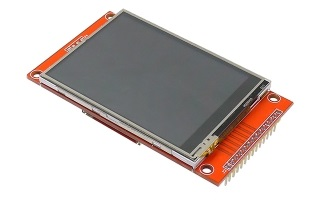
\includegraphics[width=0.7\textwidth]{./Figures/pant_LCD.png}
\caption{Pantalla LCD táctil MSP2807\protect\footnotemark.}
\label{fig:pantLCD}
\end{figure}

\footnotetext{Imagen tomada de \citep{MSP2807}}

El controlador del display utiliza una interfaz SPI para la recepción de datos y cuenta con una señal DC/RS para distinguir entre datos y registros internos. El controlador táctil también opera mediante SPI y dispone de una señal de interrupción T\_IRQ que indica cuando se ha producido una interacción en la pantalla \citep{MSP2807}.

\section{Recursos de software}

Para el firmware del microcontrolador se usaron distintas herramientas que permitieron el desarrollo de una estructura de software jerárquica, simple y eficaz.

\subsection{Sistema operativo de tiempo real FreeRTOS}

FreeRTOS es un sistema operativo de tiempo real (RTOS) diseñado para microcontroladores y microprocesadores pequeños. Se caracteriza por ser liviano, confiable y fácil de usar. Ofrece recursos como tareas, semáforos, \textit{mutexes}, colas y gestores de memoria dinámica \citep{WEBSITE:1}, lo que simplifica la creación y gestión de aplicaciones sobre el sistema operativo.

FreeRTOS se sitúa en una capa intermedia del firmware, por encima de los drivers del fabricante y debajo de la aplicación de usuario, brindando una capa de abstracción que automatiza la gestión de los recursos de hardware. Su principal ventaja es la capacidad de ejecutar múltiples tareas o procesos de manera simultánea. Esto permite estructurar aplicaciones en tareas independientes y sincronizadas \citep{WEBSITE:FREERTOS}.

\subsection{Capa de abstracción de hardware (HAL)}

Una \textit{hardware abstraction layer} o HAL es un conjunto de rutinas de software que brinda acceso a recursos de hardware a programas de aplicación. Se ubica inmediatamente por arriba del hardware y por debajo del sistema operativo que se ejecuta.

La principal ventaja de esta capa es que oculta la arquitectura del hardware del \textit{kernel} del sistema operativo. Así, el código del \textit{kernel} no tiene que ser cambiado o reescrito para que pueda correr sobre sistemas con distinto hardware y las aplicaciones de software se vuelven independientes de la plataforma (portabilidad) \citep{WEBSITE:HAL}.

La HAL de la serie de microcontroladores STM32 se denomina STM32Cube y tiene como objetivo asegurar la máxima portabilidad entre dispositivos de la misma familia y proveer APIs (\textit{Application Programming Interface}) multi-instancia para todos los periféricos (UART, SPI, temporizadores, ADC, etc.). Estas APIs están listas para usar y facilitan la implementación de la aplicación de usuario. Por ejemplo, los periféricos de comunicación cuentan con APIs para inicializarlos y configurarlos, gestionar la transferencia de datos en modo \textit{polling}, manejar las interrupciones, el DMA (\textit{Direct Memory Access}) y los errores de comunicación \citep{WEBSITE:STM32CUBE}.

\section{Periféricos utilizados}

A excepción del monitor de corriente, el resto de los periféricos utilizados ya se encuentran integrados en el chip del microcontrolador, por lo que no hubo necesidad de agregar ningún hardware adicional.

\subsection{Conversor analógico-digital (ADC)}

Un conversor analógico-digital o ADC es un dispositivo que convierte una señal eléctrica analógica proveniente, por ejemplo, de un sensor a una señal digital. De esta forma su valor puede ser almacenado en un sistema digital, por lo que estará representada por un número binario \citep{WEBSITE:2}.

\subsection{Universal Asynchronous Receiver Transmitter (UART)}

Un UART es un dispositivo utilizado para establecer una comunicación serie asíncrona, con formato de datos y velocidad de transmisión configurables. Consta solo de dos señales que conectan dos dispositivos de forma bidireccional: una para la transmisión y otra para la recepción, comúnmente llamadas TX y RX respectivamente \citep{WEBSITE:3}.

\subsection{Serial Peripheral Interface (SPI)}

SPI es una especificación de interfaz de comunicación serie sincrónica para distancias cortas. Es comúnmente utilizada para enviar datos entre un sistema embebido y pequeños periféricos como sensores y memorias SD.

Los dispositivos SPI se comunican en modo \textit{full duplex} (ambos sentidos simultáneos) y cuentan con una señal de clock, dato entrante, dato saliente y de selección de esclavo, que conecta o desconecta la operación del dispositivo con el que uno desea comunicarse. De esta forma, este estándar permite multiplexar las líneas de clock y soportar arquitecturas multi-esclavo \citep{WEBSITE:SPI}.

